%You can leave alone everything before Line 79.
\documentclass{article}
\usepackage{url,amsfonts, amsmath, amssymb, amsthm,color, enumerate}
% Page layout
\setlength{\textheight}{8.75in}
\setlength{\columnsep}{2.0pc}
\setlength{\textwidth}{6.5in}
\setlength{\topmargin}{0in}
\setlength{\headheight}{0.0in}
\setlength{\headsep}{0.0in}
\setlength{\oddsidemargin}{0in}
\setlength{\evensidemargin}{0in}
\setlength{\parindent}{1pc}
\newcommand{\shortbar}{\begin{center}\rule{5ex}{0.1pt}\end{center}}
%\renewcommand{\baselinestretch}{1.1}
% Macros for course info
\newcommand{\courseNumber}{ME 552}
\newcommand{\courseTitle}{Mechatronics}
\newcommand{\semester}{Fall 2012}
\newcommand{\xxx}[1]{\textcolor{red}{#1}}
% Theorem-like structures are numbered within SECTION units
\theoremstyle{plain}
\newtheorem{theorem}{Theorem}[section]
\newtheorem{lemma}[theorem]{Lemma}
\newtheorem{corollary}[theorem]{Corollary}
\newtheorem{proposition}[theorem]{Proposition}
\newtheorem{statement}[theorem]{Statement}
\newtheorem{conjecture}[theorem]{Conjecture}
\newtheorem{fact}{Fact}
%definition style
\theoremstyle{definition}
\newtheorem{definition}[theorem]{Definition}
\newtheorem{example}{Example}
\newtheorem{problem}[theorem]{Problem}
\newtheorem{exercise}{Exercise}
\newtheorem{algorithm}{Algorithm}
%remark style
\theoremstyle{remark}
\newtheorem{remark}[theorem]{Remark}
\newtheorem{reduction}[theorem]{Reduction}
%\newtheorem{question}[theorem]{Question}
\newtheorem{question}{Question}
%\newtheorem{claim}[theorem]{Claim}
%
% Proof-making commands and environments
\newcommand{\beginproof}{\medskip\noindent{\bf Proof.~}}
\newcommand{\beginproofof}[1]{\medskip\noindent{\bf Proof of #1.~}}
\newcommand{\finishproof}{\hspace{0.2ex}\rule{1ex}{1ex}}
\def\therefore{\boldsymbol{\text{ }
\leavevmode
\lower0.4ex\hbox{$\cdot$}
\kern-.5em\raise0.7ex\hbox{$\cdot$}
\kern-0.55em\lower0.4ex\hbox{$\cdot$}
\thinspace\text{ }}}

\newenvironment{solution}[1]{\medskip\noindent{\bf Problem #1.~}}{\shortbar}

%====header======
\newcommand{\solutions}[4]{
%\renewcommand{\thetheorem}{{#2}.\arabic{theorem}}
\vspace{-2ex}
\begin{center}
{\small  \courseNumber, \courseTitle
\hfill {\Large \bf {#1} }\\
\semester, University of Michigan, Ann Arbor \hfill
{\em Date: #3}}\\
\vspace{-1ex}
\hrulefill\\
\vspace{4ex}
{\LARGE Lab Assignment #2}\\
\vspace{2ex}
\end{center}
\begin{trivlist}
\item \textsc{Team members:\\} {#4}
\end{trivlist}
\noindent
\shortbar
\vspace{3ex}
}
% math macros
\newcommand{\defeq}{\stackrel{\textrm{def}}{=}}
\newcommand{\Prob}{\textrm{Prob}}
%==
\usepackage{graphicx}
\usepackage{xfrac}
\usepackage{amsmath}
\begin{document}
%%%%%%%%%%%%%%%%%%%%%%%%%%%%%%%%%%%%%%%%%%%%%%%%%
%\solutions{Your name}{Problem Set Number}{Date of preparation}{Collaborators}{Prover}{Verifiers}
\solutions{}{3: DC Motor Servo System}{\today}{Shiva Ghose, @gshiva\\ John Peterson, @jrpeters\\ Peter Turpel, @pturpel\\ Chan-Rong Lin, @pmelin}
%%%%%%%%%%%%%%%%%%%%%%%%%%%%%%%%%%%%%%%%%%%%%%%%%
%\renewcommand{\theproblem}{\arabic{problem}} 
%%%%%%%%%%%%%%%%%%%%%%%%%%%%%%%%%%%%%%%%%%%%%%%%%
%
% Begin the solution for each problem by
% \begin{solution}{Problem Number} and ends it with \end{solution}
%
% the solution for Problem 
\section*{Teamwork Participation Pledge :: Team 1}

I attest that I have made a fair and equitable contribution to this lab and submitted 
assignment. \\

My signature also indicates that I have followed the University of Michigan Honor Code, 
while working on this lab and assignment.\\

I accept my responsibility to look after all of the equipment assigned to me and my team, 
and that I have read and understood the X50 Lab Rules.\\

\begin{table}[h]
\begin{center}
    \begin{tabular}{|c|c|c|}
        \hline
        \textbf{Name} & \textbf{Email}     & \textbf{ \ \ \ \ \  \ \  \ \ \ \ \  \ \ Signature  \ \ \ \ \  \ \ \ \ \ \ \  \ \ } \\ \hline
        	~& ~& ~\\
	~& ~& ~\\
	Shiva Ghose   & gshiva@umich.edu   & ~                  \\
	~& ~& ~\\
	~& ~& ~\\ \hline 
	~& ~& ~\\
	~& ~& ~\\
        John Peterson & jrpeters@umich.edu & ~                  \\ 
	~& ~& ~\\
	~& ~& ~\\ \hline 
	~& ~& ~\\
	~& ~& ~\\
        Peter Turpel   & pturpel@umich.edu & ~                  \\
	~& ~& ~\\
	~& ~& ~\\ \hline 
	~& ~& ~\\
	~& ~& ~\\
        Chan-Rong Lin   & pmelin@umich.edu & ~                  \\
	~& ~& ~\\
	~& ~& ~\\ \hline 
        \hline
    \end{tabular}
\end{center}
\end{table}

\newpage

\section*{1.}

\subsection*{a.}

\subsubsection*{U1}
U1 serves as a difference circuit between $^-Ref$ and $^+Ref$ with a variable overall gain dictated by the potentiometer.

$$ V_{out} = \left( \frac{R_6}{R_5+R_6} \right) \left( \left(1 + \frac{R_2}{R_1} \right) \left( \frac{R_4}{R_3+R_4} \right) (^-Ref) - \left( \frac{R_2}{R_1} \right) (^+Ref) \right) $$
$$ V_{out} = \left( \frac{R_6}{R_5+R_6} \right) \left( \left(1+ \frac{20}{50} \right) \left( \frac{20}{50+20} \right)(^-Ref) - \left( \frac{20}{50} \right) (^+Ref) \right) $$

\begin{figure}
\begin{center}
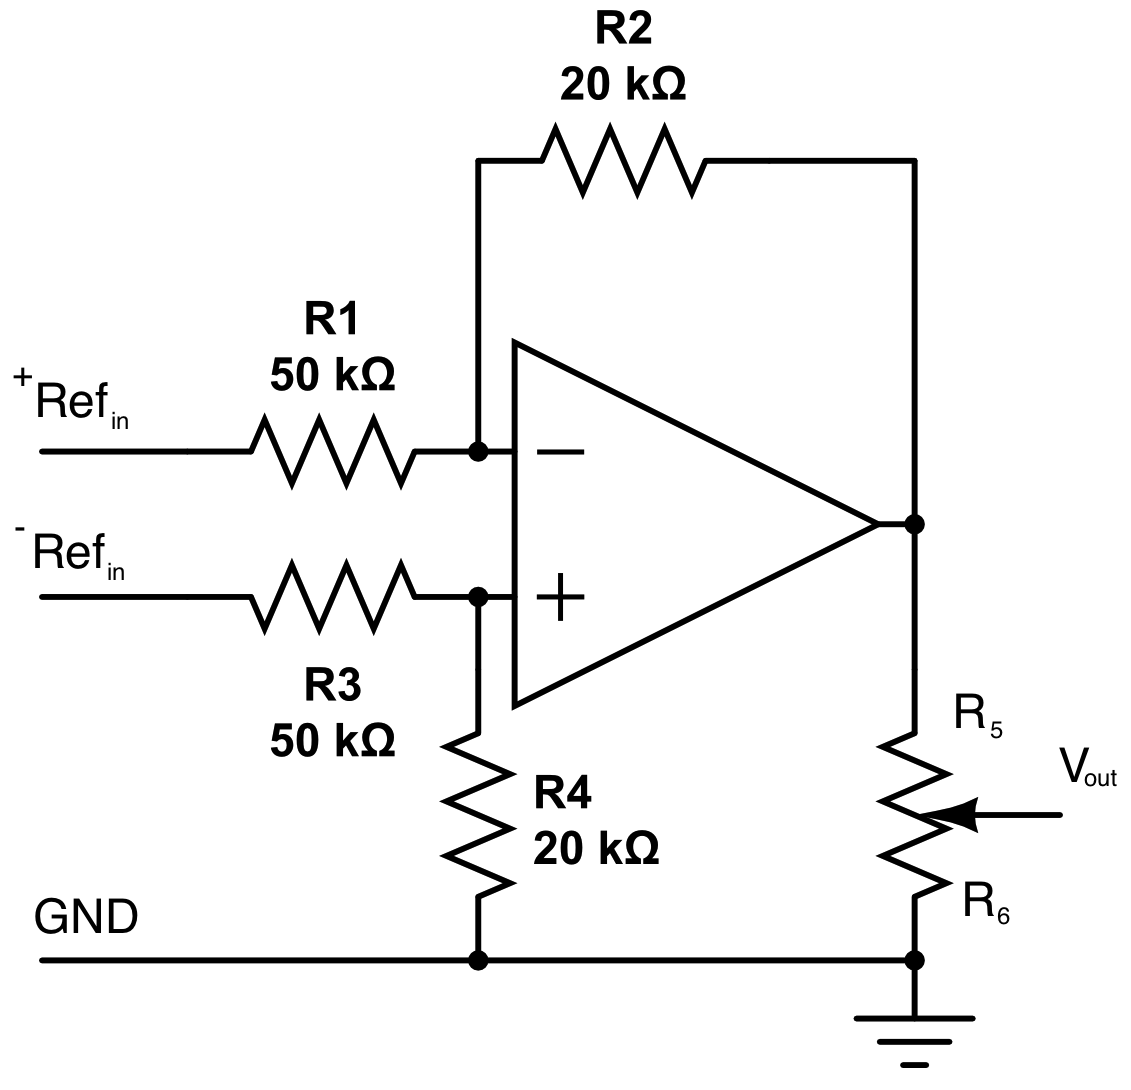
\includegraphics[width = 10cm]{q1a_u1.png}
\caption{Unit 1 within AMC servo-amplifier}
\label{q1_au1}
\end{center}
\end{figure}

\subsubsection*{U3}

U3 serves as an inverting amplifier which can be tuned by the potentiometer.

$$U3_{out} = - \left( \frac{R_3 + R_4}{R_4} \right) \left( \frac{R_2}{R_1} \right) Ref_{gain} $$
$$U3_{out} = - \left( \frac{R_3 + R_4}{R_4} \right) \left( \frac{10}{5} \right) Ref_{gain} $$

\begin{figure}
\begin{center}
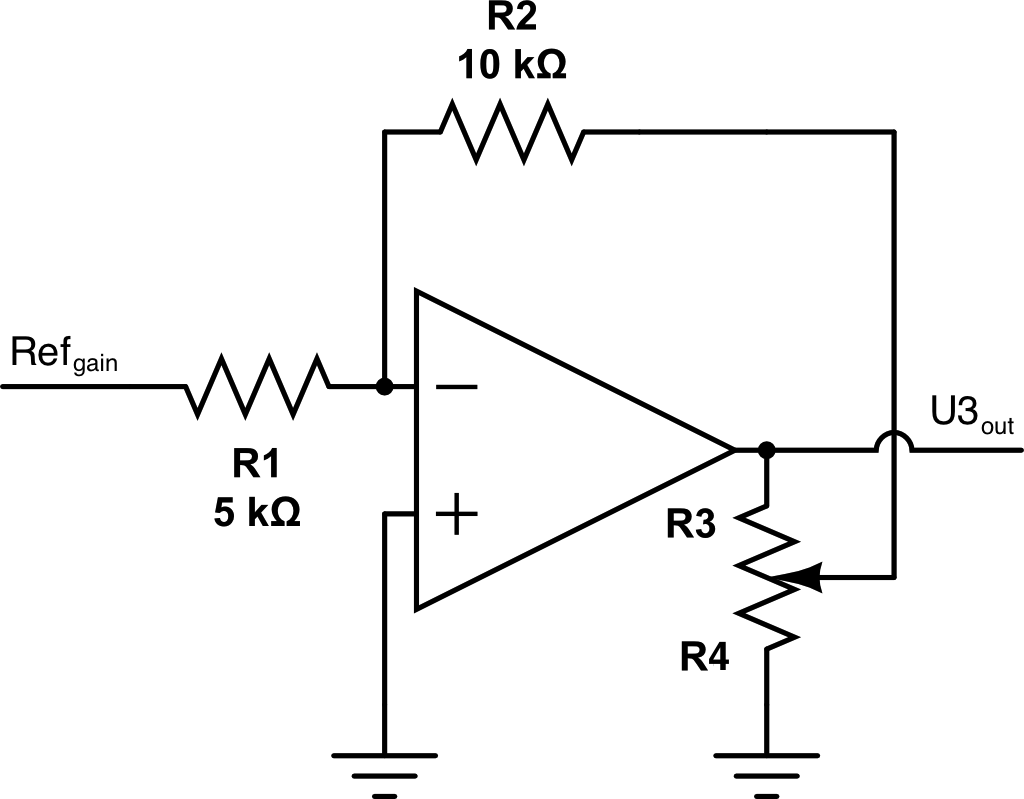
\includegraphics[width = 10cm]{q1a_u3.png}
\caption{Unit 3 within AMC servo-amplifier}
\label{q1_au3}
\end{center}
\end{figure}

\subsubsection*{U4}

$$U4_{out} = - \left( \frac{1}{R_1} \right) \left( R_2 + \frac{C_1}{s} \right) U3_{out} $$
$$U4_{out} = - \left( \frac{1}{500} \right) \left( 500 + \frac{0.01}{s} \right) U3_{out} $$

\begin{figure}
\begin{center}
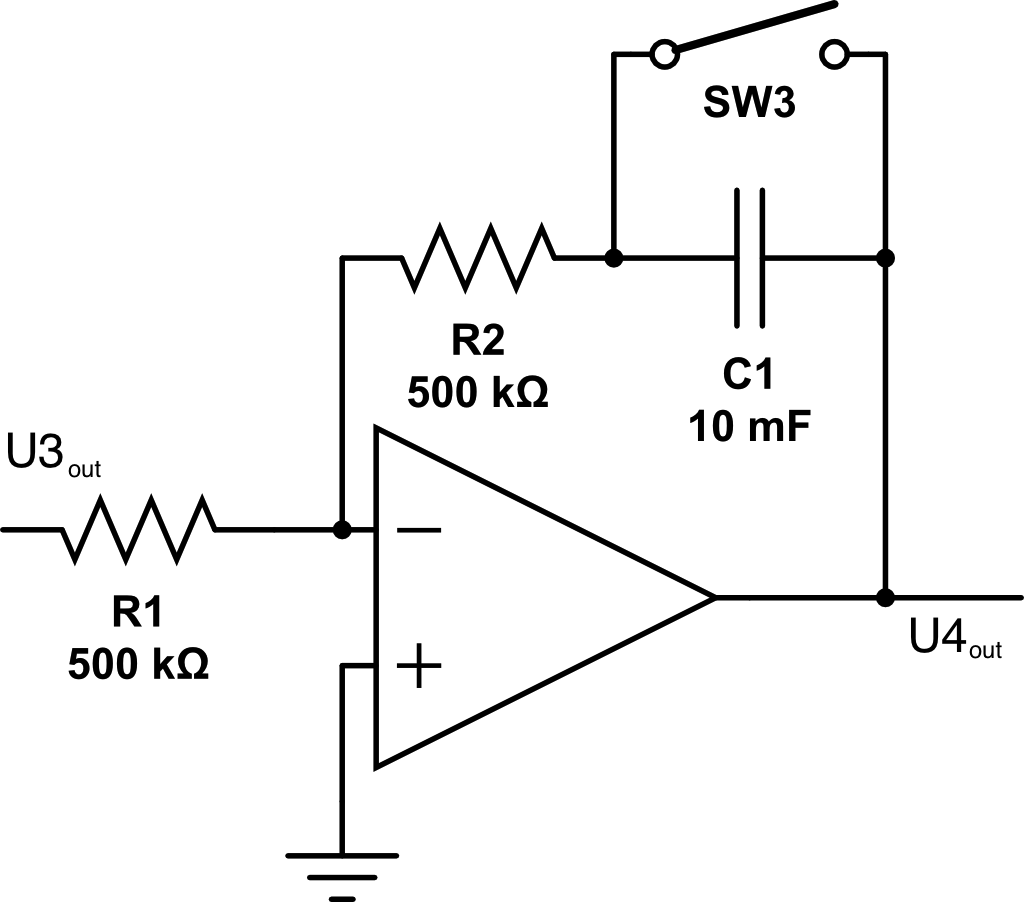
\includegraphics[width = 10cm]{q1a_u4.png}
\caption{Unit 4 within AMC servo-amplifier}
\label{q1_au4}
\end{center}
\end{figure}

\subsection*{b.}

\subsection*{c.}

\subsection*{d.}

\subsection*{e.}

\section*{2.}

\subsection*{a.}

\subsection*{b.}

\section*{3.}

\section*{4.}

\subsection*{a.}

\section*{5.}

\subsection*{a. Coulomb Friction}

\subsection*{b. Saturation}

\subsection*{c. Quantization}

\section*{6.}

\end{document}